
\documentclass[letterpaper,hide notes,xcolor={table,svgnames},pdftex,10pt]{beamer}
\def\showexamples{t}


%\usepackage[svgnames]{xcolor}

%% Demo talk
%\documentclass[letterpaper,notes=show]{beamer}

\usecolortheme{crane}
\setbeamertemplate{navigation symbols}{}

\usetheme{MyPittsburgh}
%\usetheme{Frankfurt}

%\usepackage{tipa}

\usepackage{hyperref}
\usepackage{graphicx,xspace}
\usepackage[normalem]{ulem}
\usepackage{multicol}
\usepackage{amsmath,amssymb,amsthm,graphicx,xspace}
\newcommand\SF[1]{$\bigstar$\footnote{SF: #1}}

\usepackage[default]{sourcesanspro}
\usepackage[T1]{fontenc}

\newcounter{tmpnumSlide}
\newcounter{tmpnumNote}

% old question code
%\newcommand\question[1]{{$\bigstar$ \small \onlySlide{2}{#1}}}
% \newcommand\nquestion[1]{\ifdefined \presentationonly \textcircled{?} \fi \note{\par{\Large \textbf{?}} #1}}
% \newcommand\nanswer[1]{\note{\par{\Large \textbf{A}} #1}}


 \newcommand\mnote[1]{%
   \addtocounter{tmpnumSlide}{1}
   \ifdefined\showcues {~\tiny\fbox{\arabic{tmpnumSlide}}}\fi
   \note{\setlength{\parskip}{1ex}\addtocounter{tmpnumNote}{1}\textbf{\Large \arabic{tmpnumNote}:} {#1\par}}}

\newcommand\mmnote[1]{\note{\setlength{\parskip}{1ex}#1\par}}

%\newcommand\mnote[2][]{\ifdefined\handoutwithnotes {~\tiny\fbox{#1}}\fi
% \note{\setlength{\parskip}{1ex}\textbf{\Large #1:} #2\par}}

%\newcommand\mnote[2][]{{\tiny\fbox{#1}} \note{\setlength{\parskip}{1ex}\textbf{\Large #1:} #2\par}}

\newcommand\mquestion[2]{{~\color{red}\fbox{?}}\note{\setlength{\parskip}{1ex}\par{\Large \textbf{?}} #1} \note{\setlength{\parskip}{1ex}\par{\Large \textbf{A}} #2\par}\ifdefined \presentationonly \pause \fi}

\newcommand\blackboard[1]{%
\ifdefined   \showblackboard
  {#1}
  \else {\begin{center} \fbox{\colorbox{blue!30}{%
         \begin{minipage}{.95\linewidth}%
           \hspace{\stretch{1}} Some space intentionally left blank; done at the blackboard.%
         \end{minipage}}}\end{center}}%
         \fi%
}



%\newcommand\q{\tikz \node[thick,color=black,shape=circle]{?};}
%\newcommand\q{\ifdefined \presentationonly \textcircled{?} \fi}

\usepackage{listings}
\lstset{%
  keywordstyle=\bfseries,
  aboveskip=15pt,
  belowskip=15pt,
  captionpos=b,
  identifierstyle=\ttfamily,
  escapeinside={(*@}{@*)},
  stringstyle=\ttfamiliy,
  frame=lines,
  numbers=left, basicstyle=\scriptsize, numberstyle=\tiny, stepnumber=0, numbersep=2pt}

\usepackage{siunitx}
\newcommand\sius[1]{\num[group-separator = {,}]{#1}\si{\micro\second}}
\newcommand\sims[1]{\num[group-separator = {,}]{#1}\si{\milli\second}}
\newcommand\sins[1]{\num[group-separator = {,}]{#1}\si{\nano\second}}
\sisetup{group-separator = {,}, group-digits = true}

%% -------------------- tikz --------------------
\usepackage{tikz}
\usetikzlibrary{positioning}
\usetikzlibrary{arrows,backgrounds,automata,decorations.shapes,decorations.pathmorphing,decorations.markings,decorations.text}

\tikzstyle{place}=[circle,draw=blue!50,fill=blue!20,thick, inner sep=0pt,minimum size=6mm]
\tikzstyle{transition}=[rectangle,draw=black!50,fill=black!20,thick, inner sep=0pt,minimum size=4mm]

\tikzstyle{block}=[rectangle,draw=black, thick, inner sep=5pt]
\tikzstyle{bullet}=[circle,draw=black, fill=black, thin, inner sep=2pt]

\tikzstyle{pre}=[<-,shorten <=1pt,>=stealth',semithick]
\tikzstyle{post}=[->,shorten >=1pt,>=stealth',semithick]
\tikzstyle{bi}=[<->,shorten >=1pt,shorten <=1pt, >=stealth',semithick]

\tikzstyle{mut}=[-,>=stealth',semithick]

\tikzstyle{treereset}=[dashed,->, shorten >=1pt,>=stealth',thin]

\usepackage{ifmtarg}
\usepackage{xifthen}
\makeatletter
% new counter to now which frame it is within the sequence
\newcounter{multiframecounter}
% initialize buffer for previously used frame title
\gdef\lastframetitle{\textit{undefined}}
% new environment for a multi-frame
\newenvironment{multiframe}[1][]{%
\ifthenelse{\isempty{#1}}{%
% if no frame title was set via optional parameter,
% only increase sequence counter by 1
\addtocounter{multiframecounter}{1}%
}{%
% new frame title has been provided, thus
% reset sequence counter to 1 and buffer frame title for later use
\setcounter{multiframecounter}{1}%
\gdef\lastframetitle{#1}%
}%
% start conventional frame environment and
% automatically set frame title followed by sequence counter
\begin{frame}%
\frametitle{\lastframetitle~{\normalfont(\arabic{multiframecounter})}}%
}{%
\end{frame}%
}
\makeatother

\makeatletter
\newdimen\tu@tmpa%
\newdimen\ydiffl%
\newdimen\xdiffl%
\newcommand\ydiff[2]{%
    \coordinate (tmpnamea) at (#1);%
    \coordinate (tmpnameb) at (#2);%
    \pgfextracty{\tu@tmpa}{\pgfpointanchor{tmpnamea}{center}}%
    \pgfextracty{\ydiffl}{\pgfpointanchor{tmpnameb}{center}}%
    \advance\ydiffl by -\tu@tmpa%
}
\newcommand\xdiff[2]{%
    \coordinate (tmpnamea) at (#1);%
    \coordinate (tmpnameb) at (#2);%
    \pgfextractx{\tu@tmpa}{\pgfpointanchor{tmpnamea}{center}}%
    \pgfextractx{\xdiffl}{\pgfpointanchor{tmpnameb}{center}}%
    \advance\xdiffl by -\tu@tmpa%
}
\makeatother
\newcommand{\copyrightbox}[3][r]{%
\begin{tikzpicture}%
\node[inner sep=0pt,minimum size=2em](ciimage){#2};
\usefont{OT1}{phv}{n}{n}\fontsize{4}{4}\selectfont
\ydiff{ciimage.south}{ciimage.north}
\xdiff{ciimage.west}{ciimage.east}
\ifthenelse{\equal{#1}{r}}{%
\node[inner sep=0pt,right=1ex of ciimage.south east,anchor=north west,rotate=90]%
{\raggedleft\color{black!50}\parbox{\the\ydiffl}{\raggedright{}#3}};%
}{%
\ifthenelse{\equal{#1}{l}}{%
\node[inner sep=0pt,right=1ex of ciimage.south west,anchor=south west,rotate=90]%
{\raggedleft\color{black!50}\parbox{\the\ydiffl}{\raggedright{}#3}};%
}{%
\node[inner sep=0pt,below=1ex of ciimage.south west,anchor=north west]%
{\raggedleft\color{black!50}\parbox{\the\xdiffl}{\raggedright{}#3}};%
}
}
\end{tikzpicture}
}


%% --------------------

%\usepackage[excludeor]{everyhook}
%\PushPreHook{par}{\setbox0=\lastbox\llap{MUH}}\box0}

%\vspace*{\stretch{1}

%\setbox0=\lastbox \llap{\textbullet\enskip}\box0}

\setlength{\parskip}{\fill}

\newcommand\noskips{\setlength{\parskip}{1ex}}
\newcommand\doskips{\setlength{\parskip}{\fill}}

\newcommand\xx{\par\vspace*{\stretch{1}}\par}
\newcommand\xxs{\par\vspace*{2ex}\par}
\newcommand\tuple[1]{\langle #1 \rangle}
\newcommand\code[1]{{\sf \footnotesize #1}}
\newcommand\ex[1]{\uline{Example:} \ifdefined \presentationonly \pause \fi
  \ifdefined\showexamples#1\xspace\else{\uline{\hspace*{2cm}}}\fi}

\newcommand\ceil[1]{\lceil #1 \rceil}


\AtBeginSection[]
{
   \begin{frame}
       \frametitle{Outline}
       \tableofcontents[currentsection]
   \end{frame}
}



\pgfdeclarelayer{edgelayer}
\pgfdeclarelayer{nodelayer}
\pgfsetlayers{edgelayer,nodelayer,main}

\tikzstyle{none}=[inner sep=0pt]
\tikzstyle{rn}=[circle,fill=Red,draw=Black,line width=0.8 pt]
\tikzstyle{gn}=[circle,fill=Lime,draw=Black,line width=0.8 pt]
\tikzstyle{yn}=[circle,fill=Yellow,draw=Black,line width=0.8 pt]
\tikzstyle{empty}=[circle,fill=White,draw=Black]
\tikzstyle{bw} = [rectangle, draw, fill=blue!20, 
    text width=4em, text centered, rounded corners, minimum height=2em]
    
    \newcommand{\CcNote}[1]{% longname
	This work is licensed under the \textit{Creative Commons #1 3.0 License}.%
}
\newcommand{\CcImageBy}[1]{%
	\includegraphics[scale=#1]{creative_commons/cc_by_30.pdf}%
}
\newcommand{\CcImageSa}[1]{%
	\includegraphics[scale=#1]{creative_commons/cc_sa_30.pdf}%
}
\newcommand{\CcImageNc}[1]{%
	\includegraphics[scale=#1]{creative_commons/cc_nc_30.pdf}%
}
\newcommand{\CcGroupBySa}[2]{% zoom, gap
	\CcImageBy{#1}\hspace*{#2}\CcImageNc{#1}\hspace*{#2}\CcImageSa{#1}%
}
\newcommand{\CcLongnameByNcSa}{Attribution-NonCommercial-ShareAlike}

\newenvironment{changemargin}[1]{% 
  \begin{list}{}{% 
    \setlength{\topsep}{0pt}% 
    \setlength{\leftmargin}{#1}% 
    \setlength{\rightmargin}{1em}
    \setlength{\listparindent}{\parindent}% 
    \setlength{\itemindent}{\parindent}% 
    \setlength{\parsep}{\parskip}% 
  }% 
  \item[]}{\end{list}} 




\title{Lecture  26 --- Timestamp, Validation, \& Multiversion Protocols }

\author{Jeff Zarnett \\ \small \texttt{jzarnett@uwaterloo.ca}}
\institute{Department of Electrical and Computer Engineering \\
  University of Waterloo}
\date{\today}


\begin{document}

\begin{frame}
  \titlepage

 \end{frame}


\begin{frame}
\frametitle{Concurrency via Timestamps}

We can also use timestamps for arranging concurrency. 

The timestamp, as you will recall, is a unique identifier, and they are typically assigned in the order the transactions are submitted to the system. 

If timestamps are used appropriately, then consistent results are produced without the use of any locks or locking, meaning deadlock can never occur.

\end{frame}

\begin{frame}
\frametitle{Timestamp Notation}
The notation for the timestamp of a transaction $T$ is $T\!S(T)$. 

The transactions can be ordered based on their timestamps. 

If a transaction $T_{i}$ arrives and then later another transaction $T_{j}$ arrives, then $T\!S(T_{i}) < T\!S(T_{j})$. 

If two transactions arrive at exactly the same time, then some sort of serialization procedure will be needed to make sure that they are not identical. 

It is commonly the case that the system clock is used to get the time stamp; just read the current value of the clock and use that.


\end{frame}

\begin{frame}
\frametitle{Timestamp as Logical Counter}

The alternative is a logical counter: increment a simple integer counter for each transaction. 

After a timestamp is assigned, just increment the counter. 

Eventually there is a limit (even if you can have $2^{64}$ transactions, in theory, which is quite a lot, but not infinite).

At some point the transaction counter will need to roll over or reset.

\end{frame}

\begin{frame}
\frametitle{What Are Timestamps For}

Generation of the timestamps is simple, it would seem, but what are they for? 

Timestamps are used for serializability order in the schedule. 

The system must ensure that the schedule executed is equivalent to a serial schedule in which transactions are ordered according to their timestamps.

\end{frame}

\begin{frame}
\frametitle{Read and Write Timestamps}

Every data element in the database is associated with separate timestamps for reading and writing. 

The notation can vary: they are called \textbf{read\_TS} and \textbf{write\_TS} or \textbf{r-timestamp} and \textbf{w-timestamp}. 

To save space I might personally like $T\!S_{r}$ and $T\!S_{w}$. 

Each time the a data element $X$ is read or written, its appropriate timestamp is updated to the timestamp of the transaction performing the read or write.

\end{frame}

\begin{frame}
\frametitle{Read and Write Timestamps}

The formal definition of the read timestamp of an item $X$: the largest timestamp amongst all the timestamps of transactions that have successfully read $X$. 

So $T\!S(X) = T\!S(T_{k})$ where $T_{k}$ is the youngest transaction that has read $X$ successfully.

The formal definition of the write timestamp of an item $X$: the largest timestamp amongst all the timestamps of transactions that have successfully written $X$. 

So $T\!S(X) = T\!S(T_{k})$ where $T_{k}$ is the youngest transaction that has written $X$ successfully.

\end{frame}

\begin{frame}
\frametitle{Cascading Rollback}

Unfortunately, simple timestamp ordering does not avoid the risk of cascading rollback. 

Schedules are not guaranteed to be recoverable. 

This leads us to the \alert{timestamp ordering protocol}.

\end{frame}



\begin{frame}
\frametitle{Timestamp Ordering Protocol}

For a read operation $T_{i}$ is performing on $X$:
\begin{enumerate}
	\item If $T\!S(T_{i}) < T\!S_{w}(X)$ then $T_{i}$ needs to read a value of $X$ that was already overwritten -- and therefore the read operation is not permitted and $T_{i}$ is rolled back.
	\item If $T\!S(T_{i}) \geq T\!S_{w}(X)$ the read operation is executed and $T\!S_{r}$ is set to $\max ( T\!S(T_{i}),~T\!S_{r}(X))$.
\end{enumerate}


\end{frame}


\begin{frame}
\frametitle{Timestamp Ordering Protocol}

For a write operation $T_{i}$ is performing on $X$:
\begin{enumerate}

\item If $T\!S(T_{i}) < T\!S_{r}(X)$ then the value that $T_{i}$ is producing was needed previously but the system assumed it wasn't going to happen and proceeded without it; thus the write is not permitted and $T_{i}$ is rolled back.
\item If $T\!S(T_{i}) < T\!S_{w}(X)$ then $T_{i}$ is attempting to write an obsolete value; the write is not permitted and $T_{i}$ is rolled back.
\item Otherwise, the write proceeds and $T\!S_{w}(X)$ is updated to $T\!S(T_{i})$. 

\end{enumerate}


\end{frame}

\begin{frame}
\frametitle{Restarting}

When a transaction is rolled back and restarted, the transaction is assigned a new timestamp. 

The timestamp ordering protocol does provide us with conflict serializability.

Starvation can still occur: a very long transaction might be constantly rolled back by shorter transactions constantly swooping in and making changes.

Unfortunately it might be necessary to block other transactions and let the long one finish.


\end{frame}

\begin{frame}
\frametitle{Timestamp Locking Protocol}

In the example below, transaction $T_{25}$ reads values $A$ and $B$ , and transaction $T_{26}$ modified both $A$ and $B$:

\begin{center}
	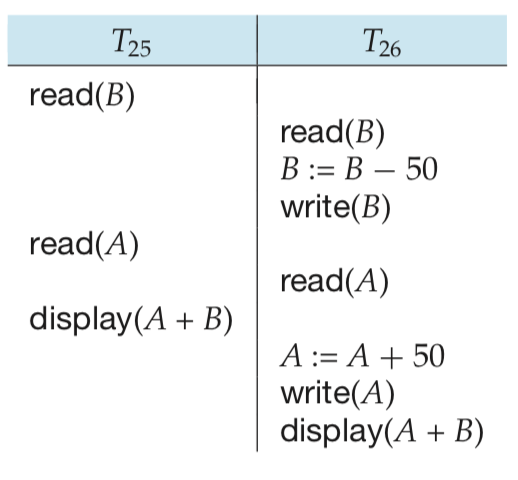
\includegraphics[width=0.3\textwidth]{images/timestamp-schedule}
\end{center}

It is worth noting that neither two phase locking nor the simple timestamp ordering protocol covers all serializable schedules.


\end{frame}

\begin{frame}
\frametitle{Strict Timestamp Ordering}
If we would like to recoverability we can have strict timestamp ordering. 

$T_{i}$ that issues a read or write of $X$ where $T\!S(T_{i}) > T\!S_{w}(X)$, then the read or write is delayed until the transaction that last wrote $X$ has committed or aborted. 

This, in some way, requires simulating locking item $X$ until a previous write has been committed or aborted.

There cannot be a deadlock because a transaction can only wait on an older transaction (one with a lower timestamp).

\end{frame}

\begin{frame}
\frametitle{Thomas's Write Rule}
A modification of the basic algorithm called Thomas's Write Rule allows greater concurrency than the basic algorithm and also, hopefully, rejects fewer writes. 

To explain it simply, it is ``ignore outdated writes''.

More formally, the write item checks are modified to the following;
\begin{enumerate}
	\item If $T\!S_{r}(X) > T\!S(T_{i})$ then abort and roll back $T_{i}$ (write rejected).
	\item If $T\!S_{w}(X) > T\!S(T_{i})$, then do not execute the write, but continue executing (do not roll back the transaction).
	\item Otherwise, the write proceeds and $T\!S_{w}(X)$ is updated to $T\!S(T_{i})$. 
\end{enumerate}

\end{frame}

\begin{frame}
\frametitle{Validation Based Protocol}

A transaction that is read-only does not interfere with any other read-only transaction. 

If a database has many more reads than writes, then a concurrency control routine might do unnecessary work or delay transactions unnecessarily.

If we could instead just step in where transactions may be in conflict, that would be better. 

It is necessary then to find out what transactions are the ones that have the potential for conflict...


\end{frame}

\begin{frame}
\frametitle{Validation Protocol}

Transactions have three phases (although read only transactions skip the last one). 

\begin{enumerate}
	\item \textbf{Read Phase.} 
	\item \textbf{Validation Phase.} 
	\item \textbf{Write Phase.} 
\end{enumerate}

\end{frame}

\begin{frame}
\frametitle{Validation Test}

The validation test for the current transaction $T_{i}$, for each transaction $T_{k}$ where $T\!S(T_{k}) < T\!S(T_{i})$, one of the following conditions must hold:

\begin{enumerate}
	\item $T_{k}$ finishes before the start of $T_{i}$: serializability order is maintained because the current transaction starts after the previous one finished.
	\item The set of data items written by $T_{k}$ does not intersect with the set of data items read by $T_{i}$, and $T_{k}$ finishes writing before $T_{i}$ starts its validation phase. This ensures that the writes of these transactions do not overlap.
\end{enumerate} 

\end{frame}

\begin{frame}
\frametitle{Validation Protocol}

To make this work out as expected we need, now, three timestamps for each transaction. 

One for the start of the transaction, one for the start of the validation phase, and then a final timestamp for when the transaction is finished.

Validation prevents cascading rollbacks because the writes don't really take place until the validation phase has taken place.

This is called \alert{optimistic concurrency control}: transactions assume they will finish. 

The locking and timestamp approaches re a bit more pessimistic. They force a rollback if there is a risk of conflict.

\end{frame}



\begin{frame}
\frametitle{The glass is full with a Factor of Safety of 2}

That potentially leads to an interesting discussion on the subject of whether an optimistic or pessimistic type approach is better.

The general recommendation is that optimistic approaches are lower overhead and better for situations where we expect there is not much contention.

\begin{center}
	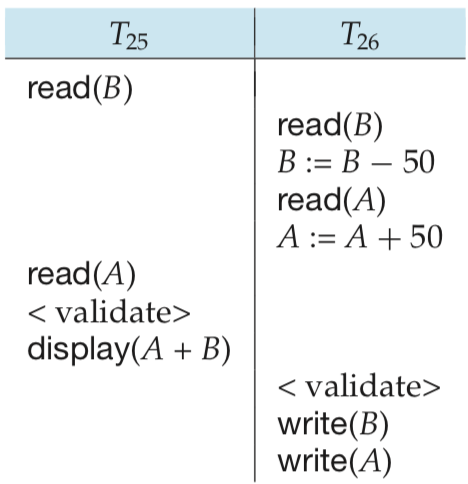
\includegraphics[width=0.3\textwidth]{images/validation}
\end{center}

\end{frame}

\begin{frame}
\frametitle{Multiversion Schemes}

Thus far we have said that a transaction must be either delayed or denied (aborted) to ensure serializability. 

In a multiversion scheme, we have multiple versions of the data at the same time.

Instead of rejecting a read because a write has taken place in the meantime, the read is provided an older version of the item. 

Choosing which one is meant to be read is the hard part of this routine.
\end{frame}

\begin{frame}
\frametitle{Keeping Extra Data}
This does require more storage space to maintain multiple versions of the data. 

Old versions might be maintained anyway for recovery, or just record keeping purposes.

Many databases are used in environments where all changes must be tracked for legal reasons.

\end{frame}


\begin{frame}
\frametitle{Multiversion Seralizability}


Ensuring serializability requires holding to just two rules:

\begin{enumerate}
	\item If transaction $T$ tries to write item $X$, and version $i$ of $X$ has the highest write timestamp of all versions of $X$ that is also less than or equal to the timestamp of $T$, and the read timestamp of $X_{i}$ is larger than the timestamp of $T$, the abort the transaction $T$ and roll it back. Otherwise, create a new version of $X$ with read and write timestamps equal to the timestamp of $T$.
	
	\item If transaction $T$ wants to read item $X$, find the version of $X$ ($X_{i}$) that has the highest write timestamp of all versions of $X$ that is also less than or equal to the timestamp of $T$. Update the read timestamp of $X_{i}$ to the maximum of its current read timestamp and the timestamp of $T$.
\end{enumerate}


\end{frame}

\begin{frame}
\frametitle{Reading is Succeeding}
The goal is that read operations are always successful, even if they read an older version. 

A write, however, might not be permitted if it comes ``too late'' -- trying to write a version that another transaction would have read. 

The drawback is that every read requires us to update the read timestamp, which is itself a write operation (and may result in a disk access).

\end{frame}

\begin{frame}
\frametitle{Cleaning Up}

When do we know that we can get rid of an old version? 

An old version is no longer needed when its write timestamp is younger than that of the oldest transaction in the system. 

But one must be careful then to only delete old versions; at least the current version must be maintained. 

But also it means that in a period in which there are no transactions active, we may clean up any old versions. 

That may not occur frequently enough in a heavily used database, so it might be a periodic task to simply trash very old versions.

We resolve any conflicts on writes through rollbacks, which are expensive, rather than through waiting.

\end{frame}

\begin{frame}
\frametitle{Multiversion Two Phase Locking}

What if we said we want an all-of-the-above solution that combines two phase locking with the multiversion scheme? 

The advantage of multiversion schemes is that reads don't fail. 

The advantage of two phase locking is that locks allow transactions to wait rather than roll back, and deadlock is avoided. 

The plan is to allow each transaction to be handled in the way they like best. 

Thus, read-only transactions are differentiated from the update transactions.


\end{frame}


\begin{frame}
\frametitle{Update Transactions}
Update transactions use two phase locking, with the restriction that they hold locks up until the end of the transaction. 

There his only one timestamp for the transaction, which is used to both serialize the transactions and to assign the version of the data written.

The timestamp under this scheme is an incrementing counter rather than the actual time of the transaction. 

\end{frame}

\begin{frame}
\frametitle{Read-Only Transactions}
Read-only transactions are assigned a timestamp based on the current value of the counter for update transactions, at the time when the read transaction is created. 

Multiple read transactions can have the same value of their timestamp. 

In effect, the read transaction's timestamp $k$ is declaring that its view of the data is the version at time $k$. 

A transaction that reads some data $X$ with its timestamp $k$ gets the version of $X$ with the largest timestamp less than or equal to $k$. 

\end{frame}

\begin{frame}
\frametitle{Multiversion Transactions}
If an update transaction wants to read an item, it acquires a shared lock on the latest version of the item.

To do an update it acquires an exclusive lock and creates a new version of that item with the timestamp being the maximum value (effectively: infinity)

The new version has this infinite timestamp so it won't be read by any read transaction, but it will be overwritten when the write transaction commits.

This does mean that only one transaction can commit at a time.

\end{frame}















\end{document}

